% Figures — included after results section
\begin{figure}[t]
  \centering
  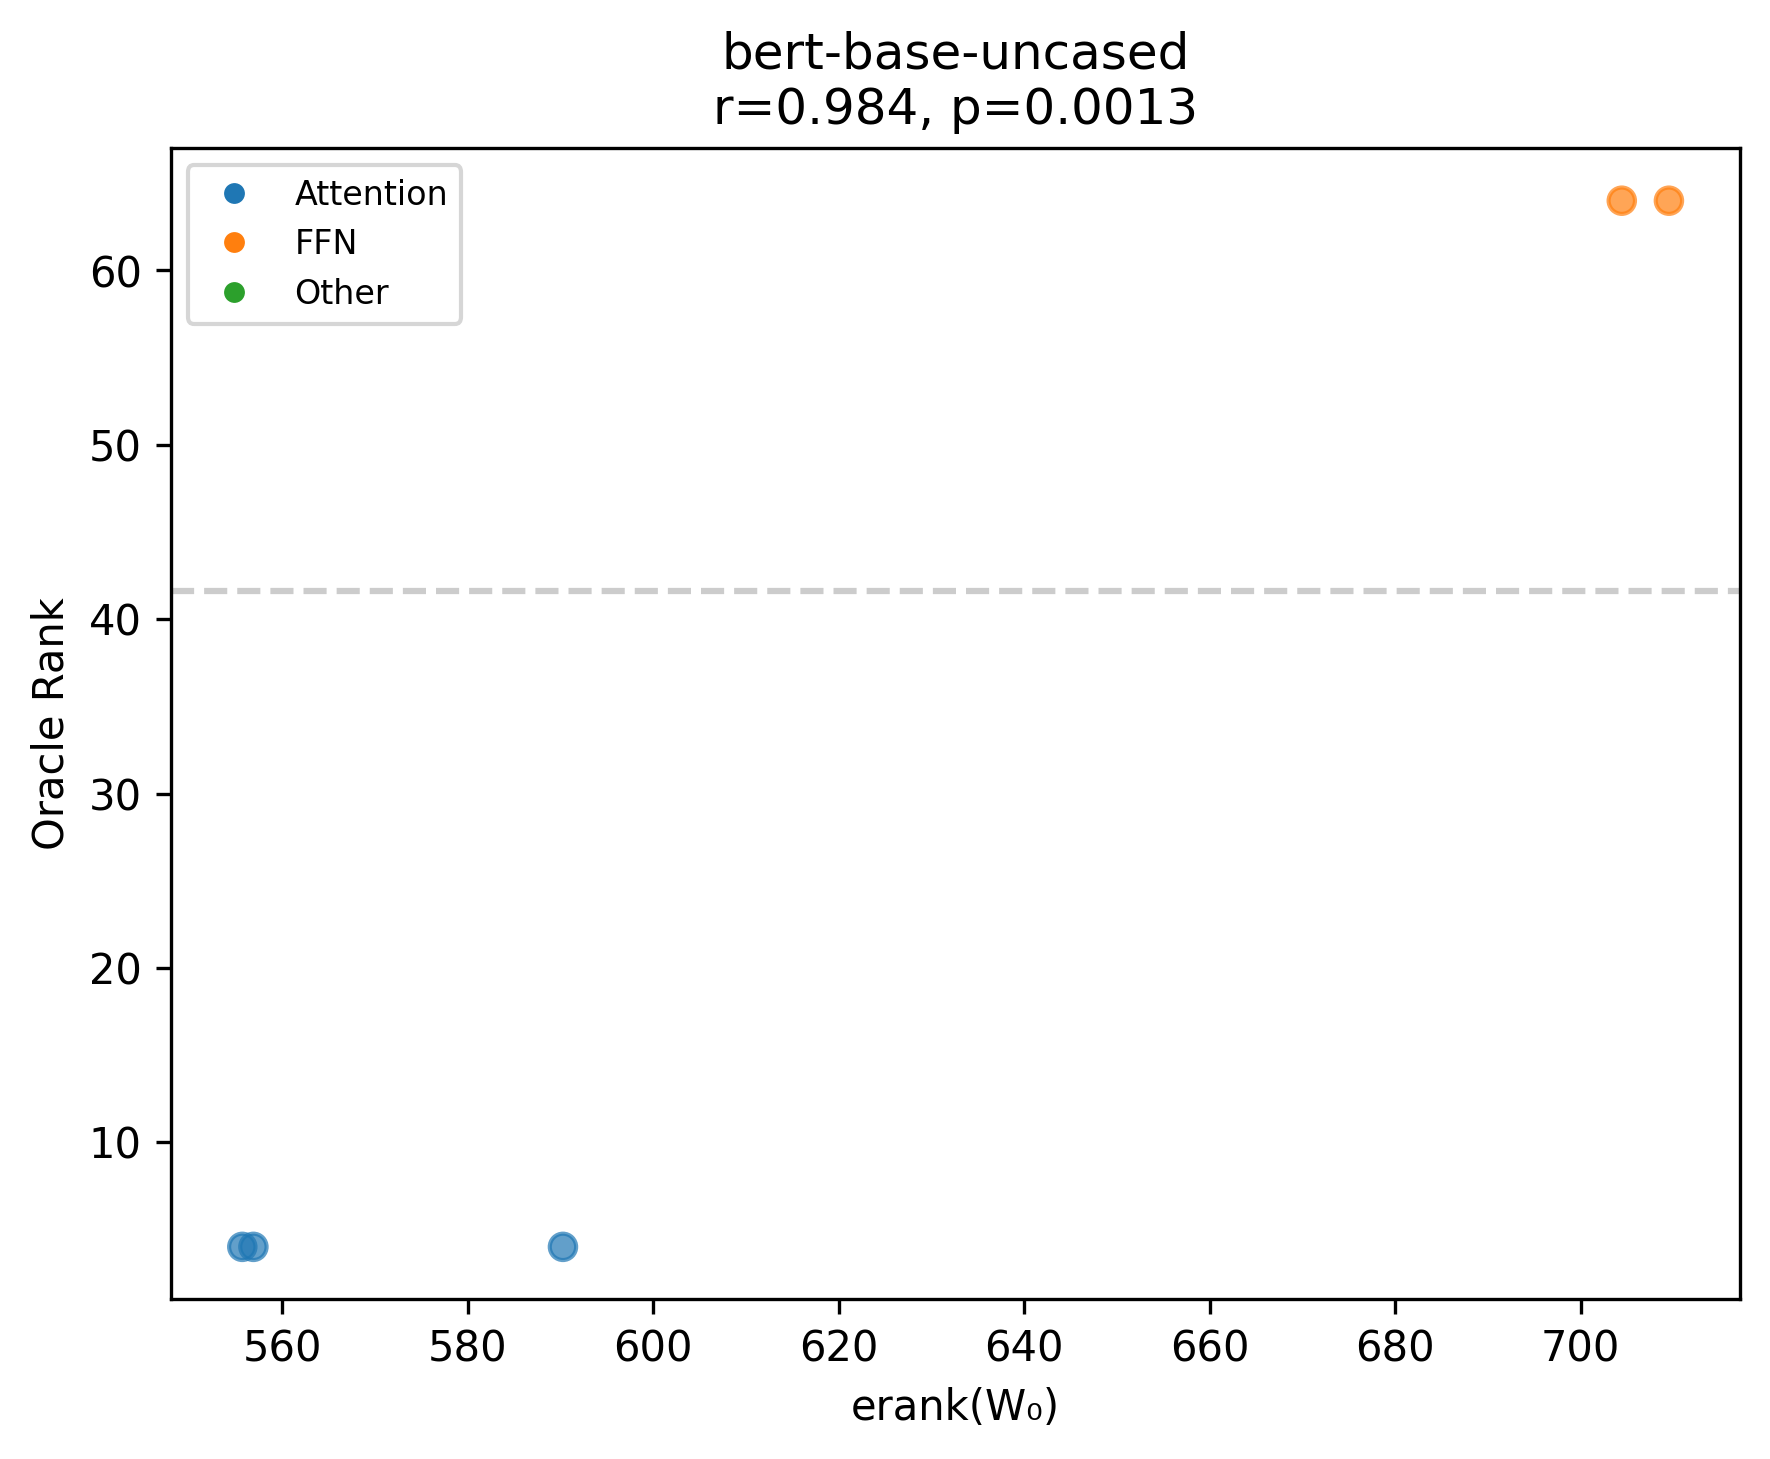
\includegraphics[width=\columnwidth]{figures/scatter_erank_vs_oracle}
  \caption{erank($W_0$) vs.\ PARA oracle rank for 5 BERT-base-uncased layers. Attention layers (erank $\sim$557--590) receive oracle rank 4; FFN intermediate layers (erank $\sim$704--710) receive oracle rank 64. Pearson $r = 0.984$.}
  \label{fig:scatter}
\end{figure}

\begin{figure}[t]
  \centering
  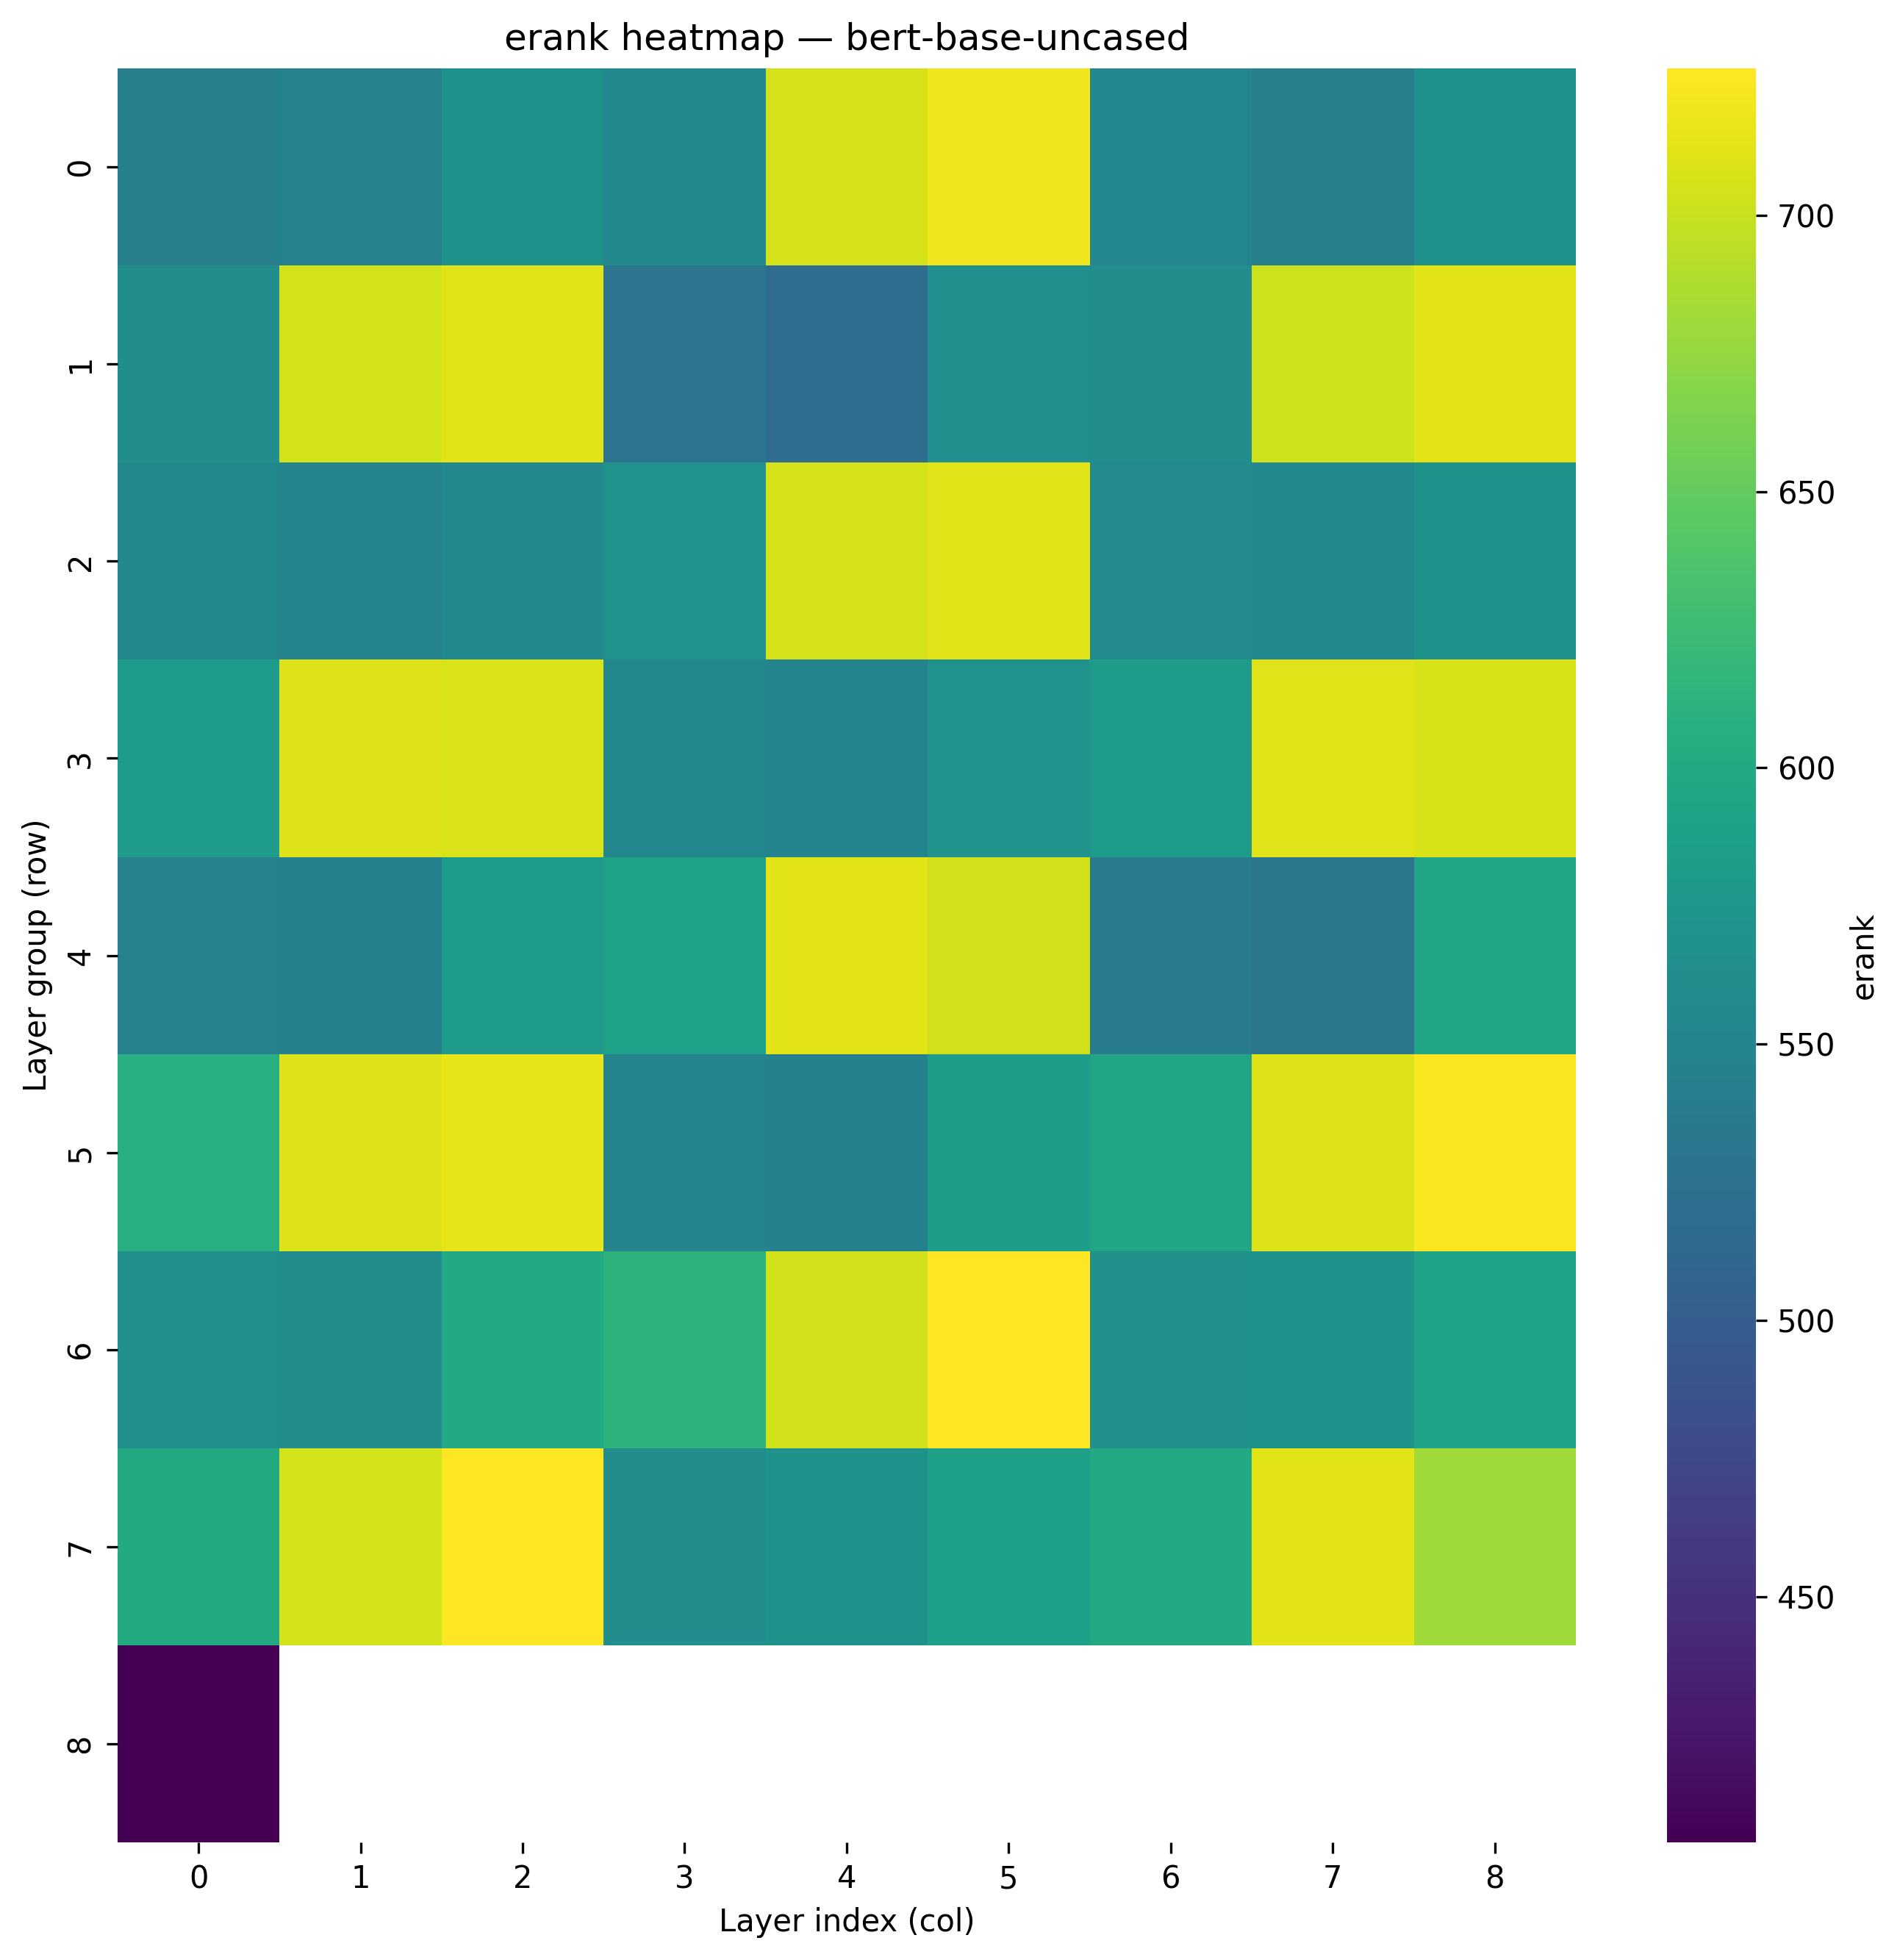
\includegraphics[width=\columnwidth]{figures/erank_heatmap_bert-base-uncased}
  \caption{erank heatmap for BERT-base-uncased (72 LoRA-targetable layers). FFN intermediate/output layers consistently show higher erank ($\sim$700--726) than attention Q/K/V/O layers ($\sim$530--611).}
  \label{fig:heatmap}
\end{figure}

\begin{figure}[t]
  \centering
  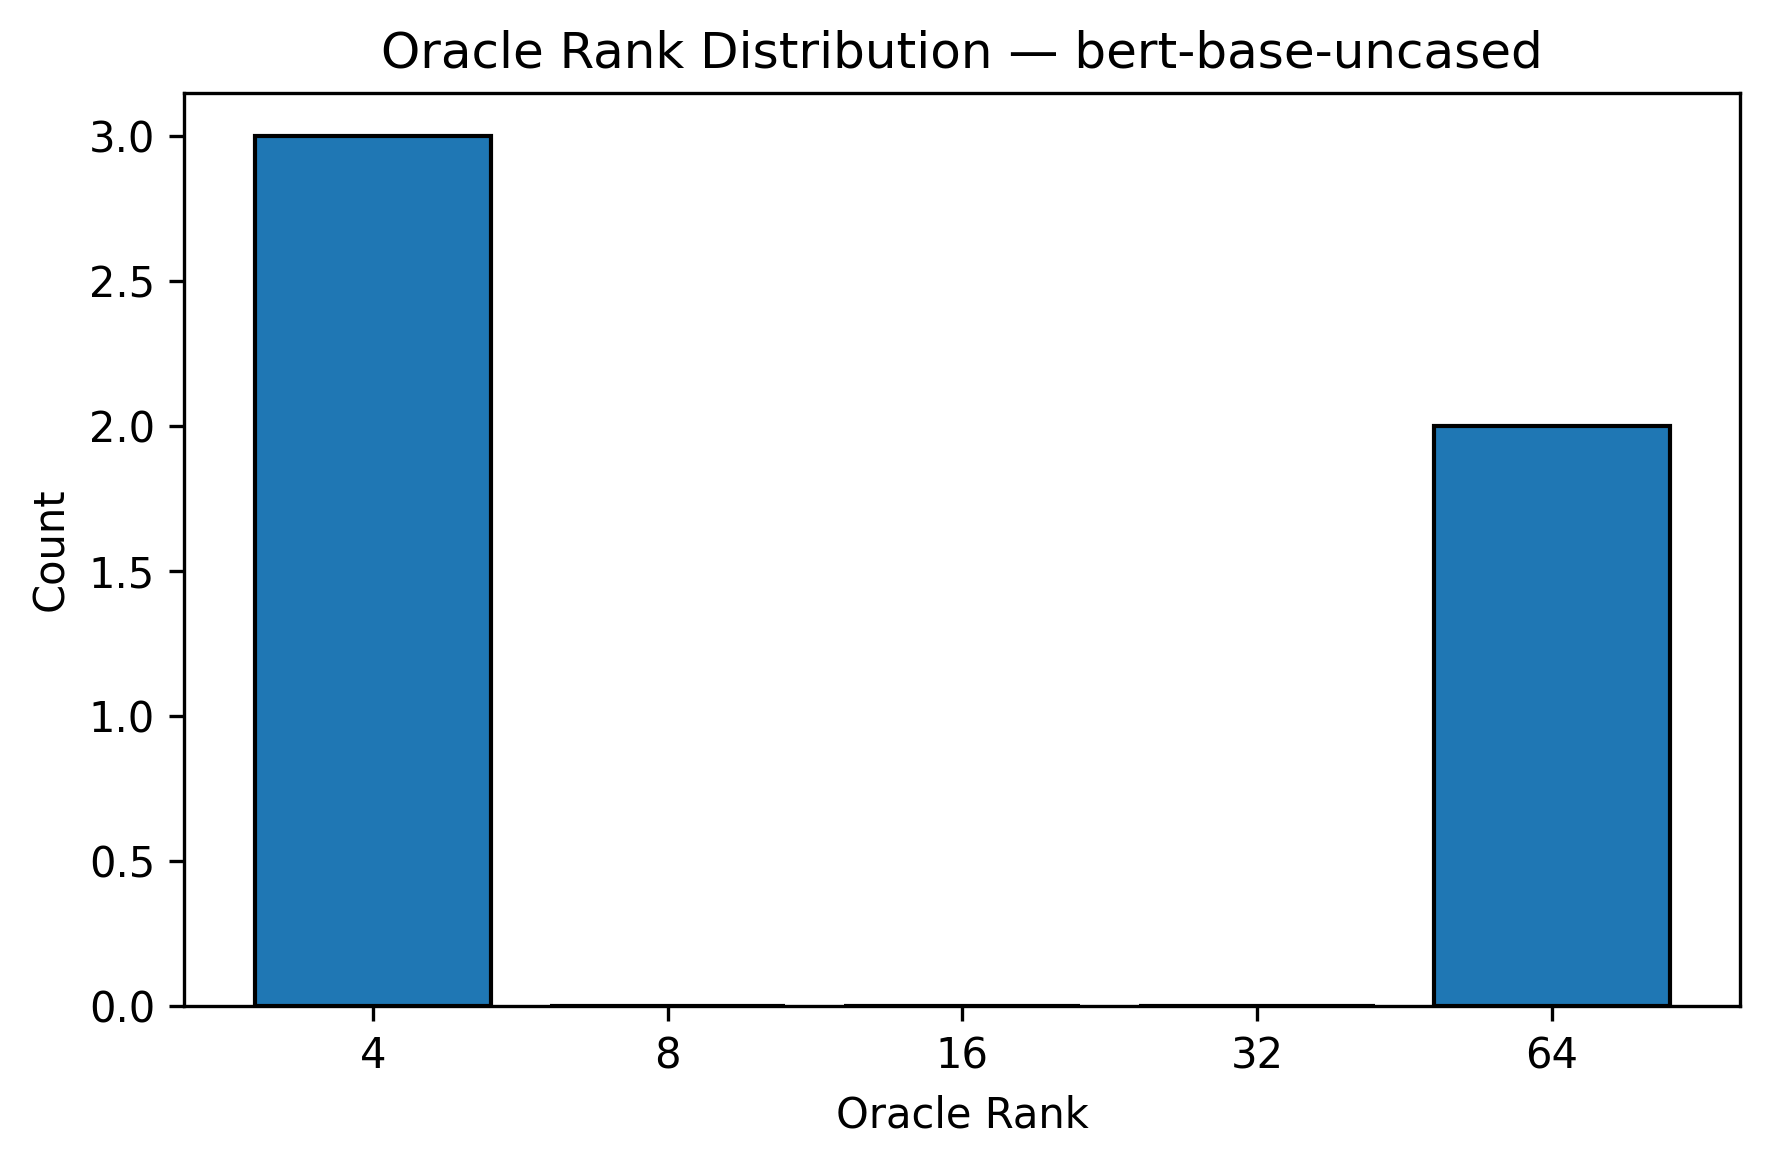
\includegraphics[width=\columnwidth]{figures/oracle_hist_bert-base-uncased}
  \caption{Distribution of PARA oracle ranks for 5 measured BERT-base-uncased layers. The oracle assigns exclusively $r^* = 4$ (attention layers) or $r^* = 64$ (FFN intermediate layers), revealing a bimodal structure.}
  \label{fig:oracle_hist}
\end{figure}

\begin{figure}[t]
  \centering
  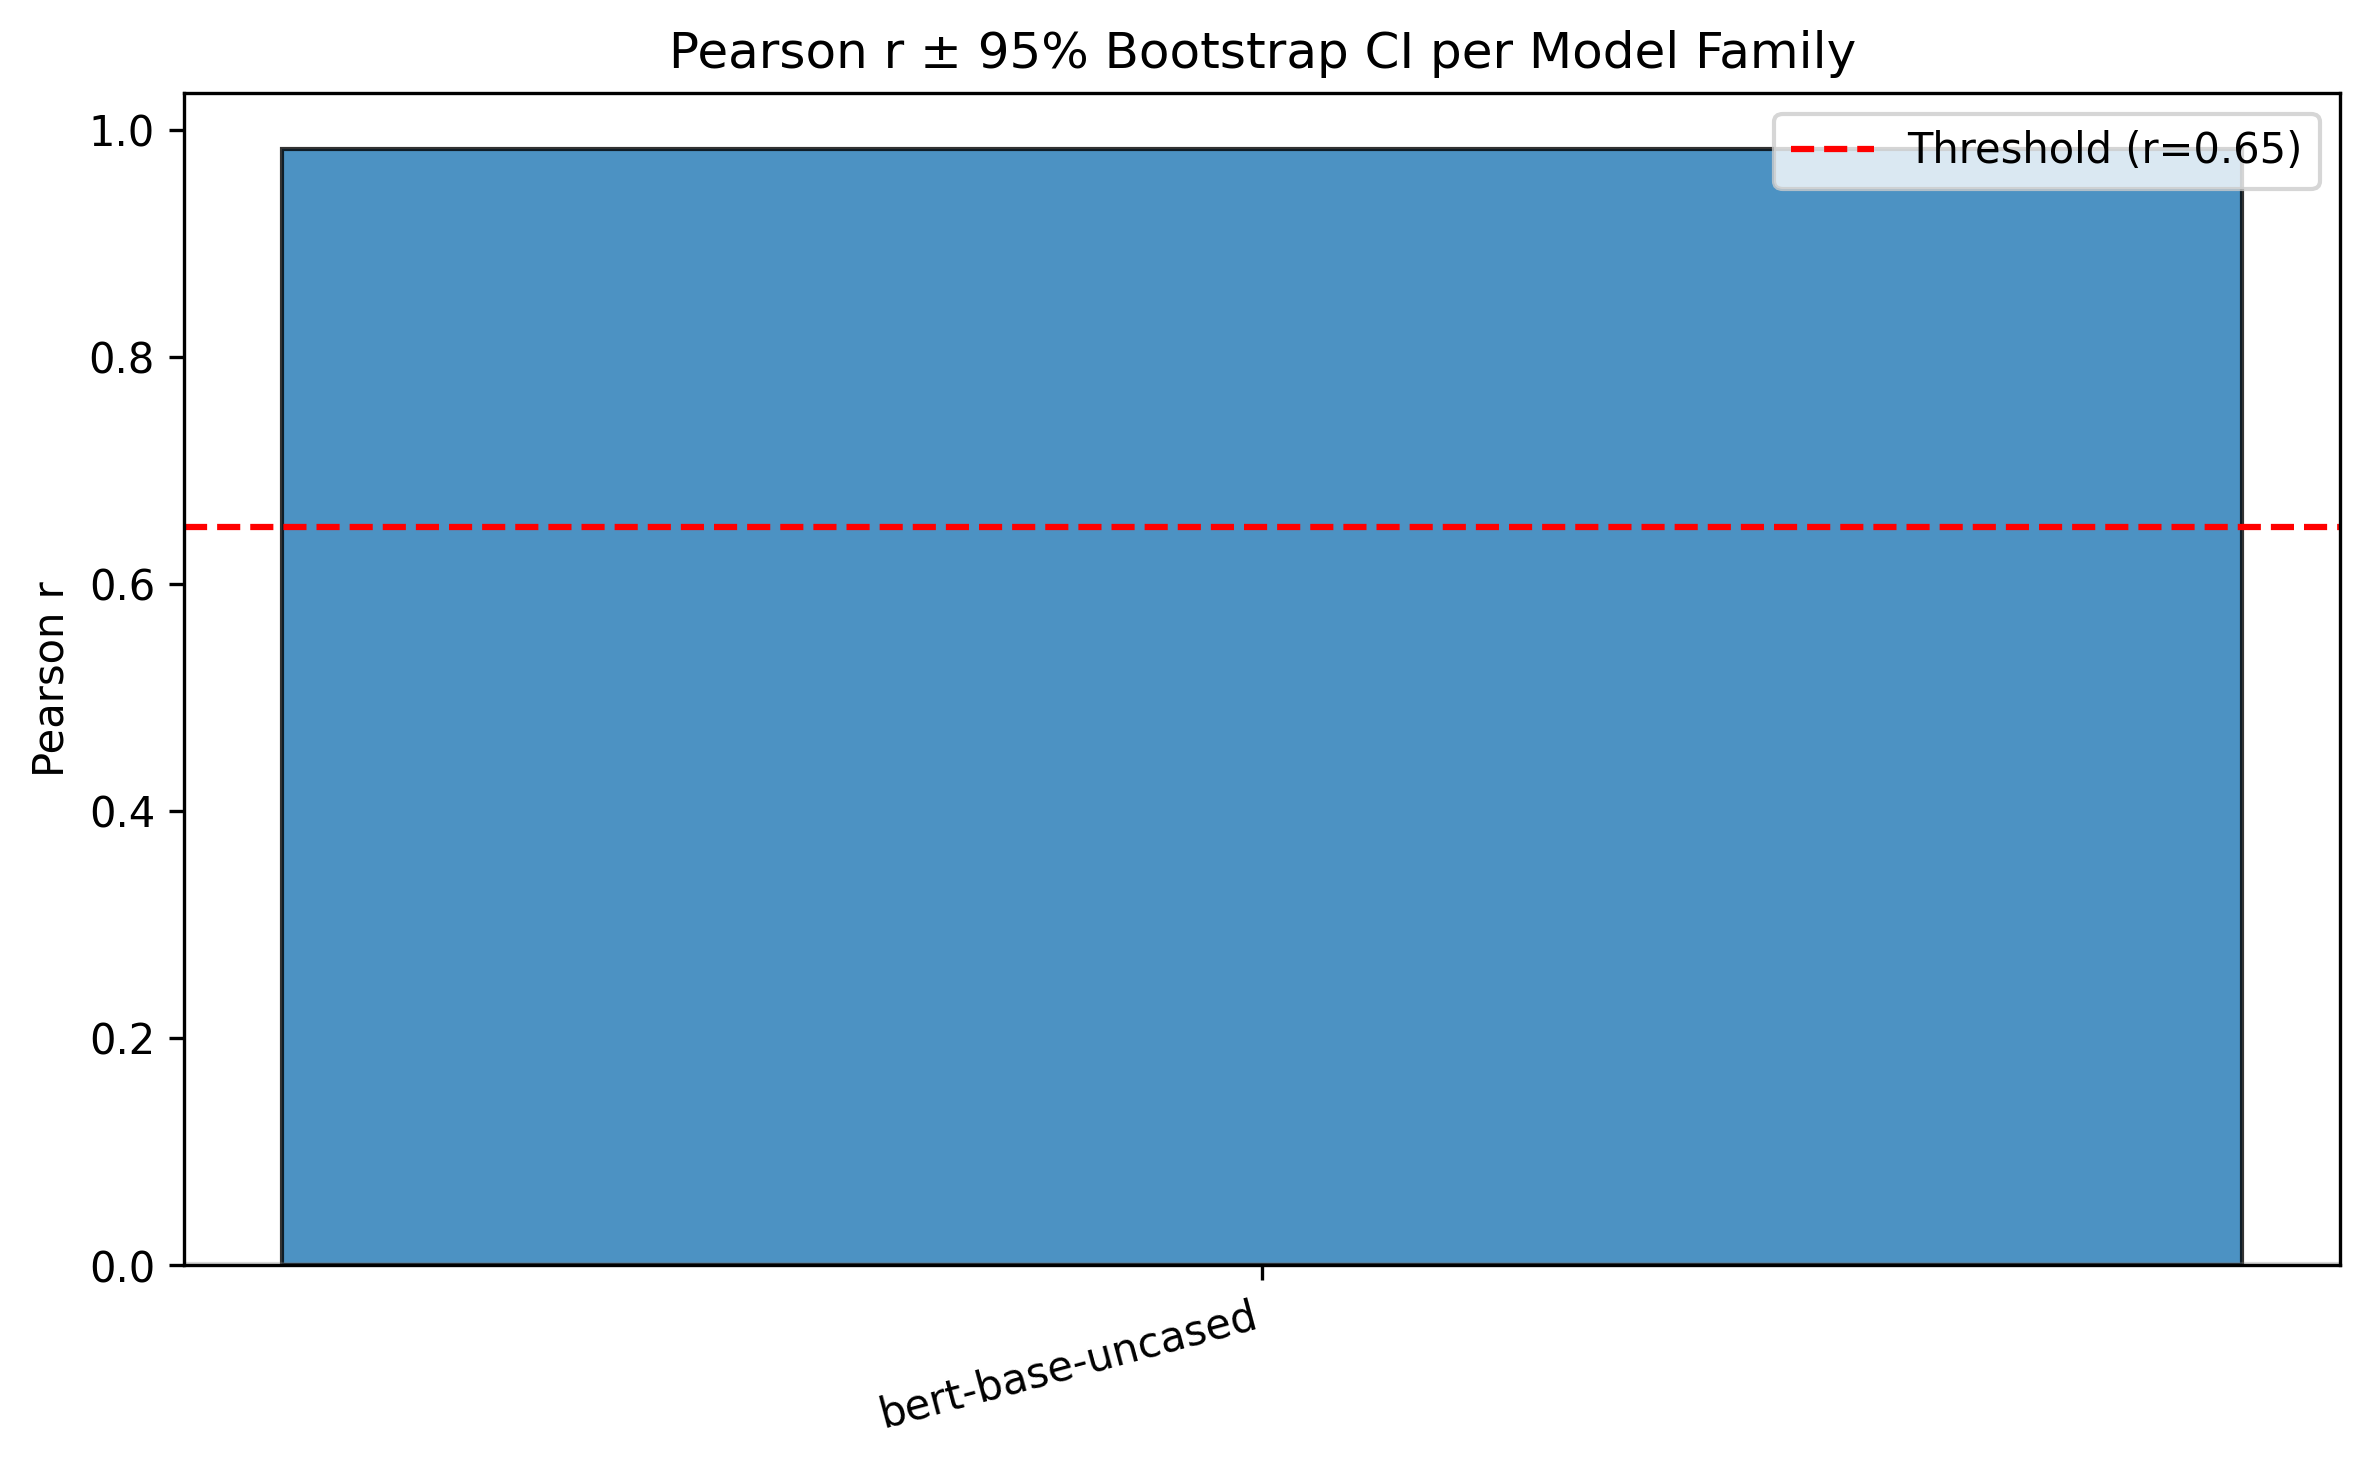
\includegraphics[width=\columnwidth]{figures/bootstrap_ci}
  \caption{Bootstrap confidence intervals for the erank--oracle Pearson correlation. Note: CI computation returned NaN at $n=5$ due to the degenerate bimodal structure; shown for completeness.}
  \label{fig:bootstrap}
\end{figure}
